\section*{Задача 4.2}
\subsection*{Постановка задачи}

Дана функция $y = f(x)$. Приблизить функцию методом интерполяции, используя многочлен Лагранжа. Степень $n$ подобрать таким образом, чтобы максимальная величина погрешности на отрезке $[a, b]$ не превышала заданной величины $\varepsilon$. Построить графики многочленов и графики погрешностей. Приблизить функцию методом интерполяции, указанным в индивидуальном варианте (Квадратичный сплайн с дополнительным условием $y'(a) = f'(a)$). Сравнить полученные результаты.
\begin{gather}
	f(x) = x\sin{(2 - x)}, [1, 4] \\
	\varepsilon = 0.001
\end{gather}
	
\subsection*{Теоретический материал}

Так как имеется свобода выбора отрезков разбиения, то имеет смысл выбрать точки таким образом, чтобы погрешность интерполяции была минимальной. Для этого воспользуемся свойством наименее уклонятся от нуля на отрезке $[-1, 1]$ многочленов Чебышева. То есть в качестве узлов интерполяции возьмем нули многочлена Чебышева:

\[
	x_k = \dfrac{a + b}{2} + \dfrac{b - a}{2}\cos{\left(\pi\dfrac{2k + 1}{2n + 2}\right)}, k = 0, 1\dots, n
\]

\textbf{Определение}{
	Сплайном степени $m$ называется функция $S_m(x)$, обладающая следующими свойствами:
	\begin{enumerate}
		\item Функция $S_m(x)$ непрерывна на $[a, b]$ со своими производными.
		\item На каждом отрезке $[x_i, x_{i+1}]$ функция $S_m(x)$ совпадает с некоторым алгебраическим многочленом $P_{m, i}(x)$ степени $m$.
		\item $S_m(x_i) = y_i$, $i = 0, 1\dots n$
	\end{enumerate}
}

\textbf{Определение}{
	Величина $R_n(x) = |f(x) - P_n(x)|$ называется остаточным членом
интерполяции или погрешностью интерполяции.
}

\textbf{Теорема}{
	Пусть функция $f(x)$ дифференцируема $(n+1)$ раз на отрезке $[a, b]$, содержащем узлы интерполяции $x_i$. Тогда для погрешности интерполяции в точке $x \in [a, b]$ справедлива оценка:
	\[
		R_n(x) = |f(x) - P_n(x)| \leq \dfrac{M_{n+1}}{(n+1)!}|\omega_{n+1}(x)|
	\]
	Где $M_{n+1} = max|f^{(n+1)}(x)|$, а $\omega_{n+1}(x) = (x - x_0)\dots(x - x_n)$
}

\subsection*{Решение}

Коэффициенты многочленов сплайна будем искать следующим образом:

\begin{enumerate}
	\item Запишем многочлены в форме $P_i(x) = a_i + b_i(x - x_i) + c_i(x - x_i)(x - x_{i+1})$.
	\item Из условий интерполяции получаем: $a_i = f(x_i)$ а также $a_i + b_i(x_{i+1} - x_i) = a_{i+1} = f(x_{i+1})$, то есть $b_i = \dfrac{a_{i+1} - a_i}{x_{i+1} - x_i}$.
	\item Коэффициенты $c_i$ будем определять из условий непрерывности производной: $P_i'(x_{i+1}) = P_{i+1}'(x_{i+1})$. То есть: $b_i - 2c_ix_i = b_{i+1} - 2x_{i+2}c_{i+1}$. В конечном итоге получаем следующую формулу для $c_{i+1}$: $c_{i+1} = \dfrac{b_{i+1} - b_i}{2x_{i+2}} + \dfrac{x_i}{x_{i+2}}c_i$.
\end{enumerate}

\subsection*{Анализ результатов}

Анализ графиков погрешности показал, что выбор узлов интерполяции согласованно с нулями многочленов Чебышева дает значительный прирост в точности для глобальной интерполяции функции на отрезке с помощью многочлена в форме Лагранжа при $n = 7$(см. рис.) 

\noindent
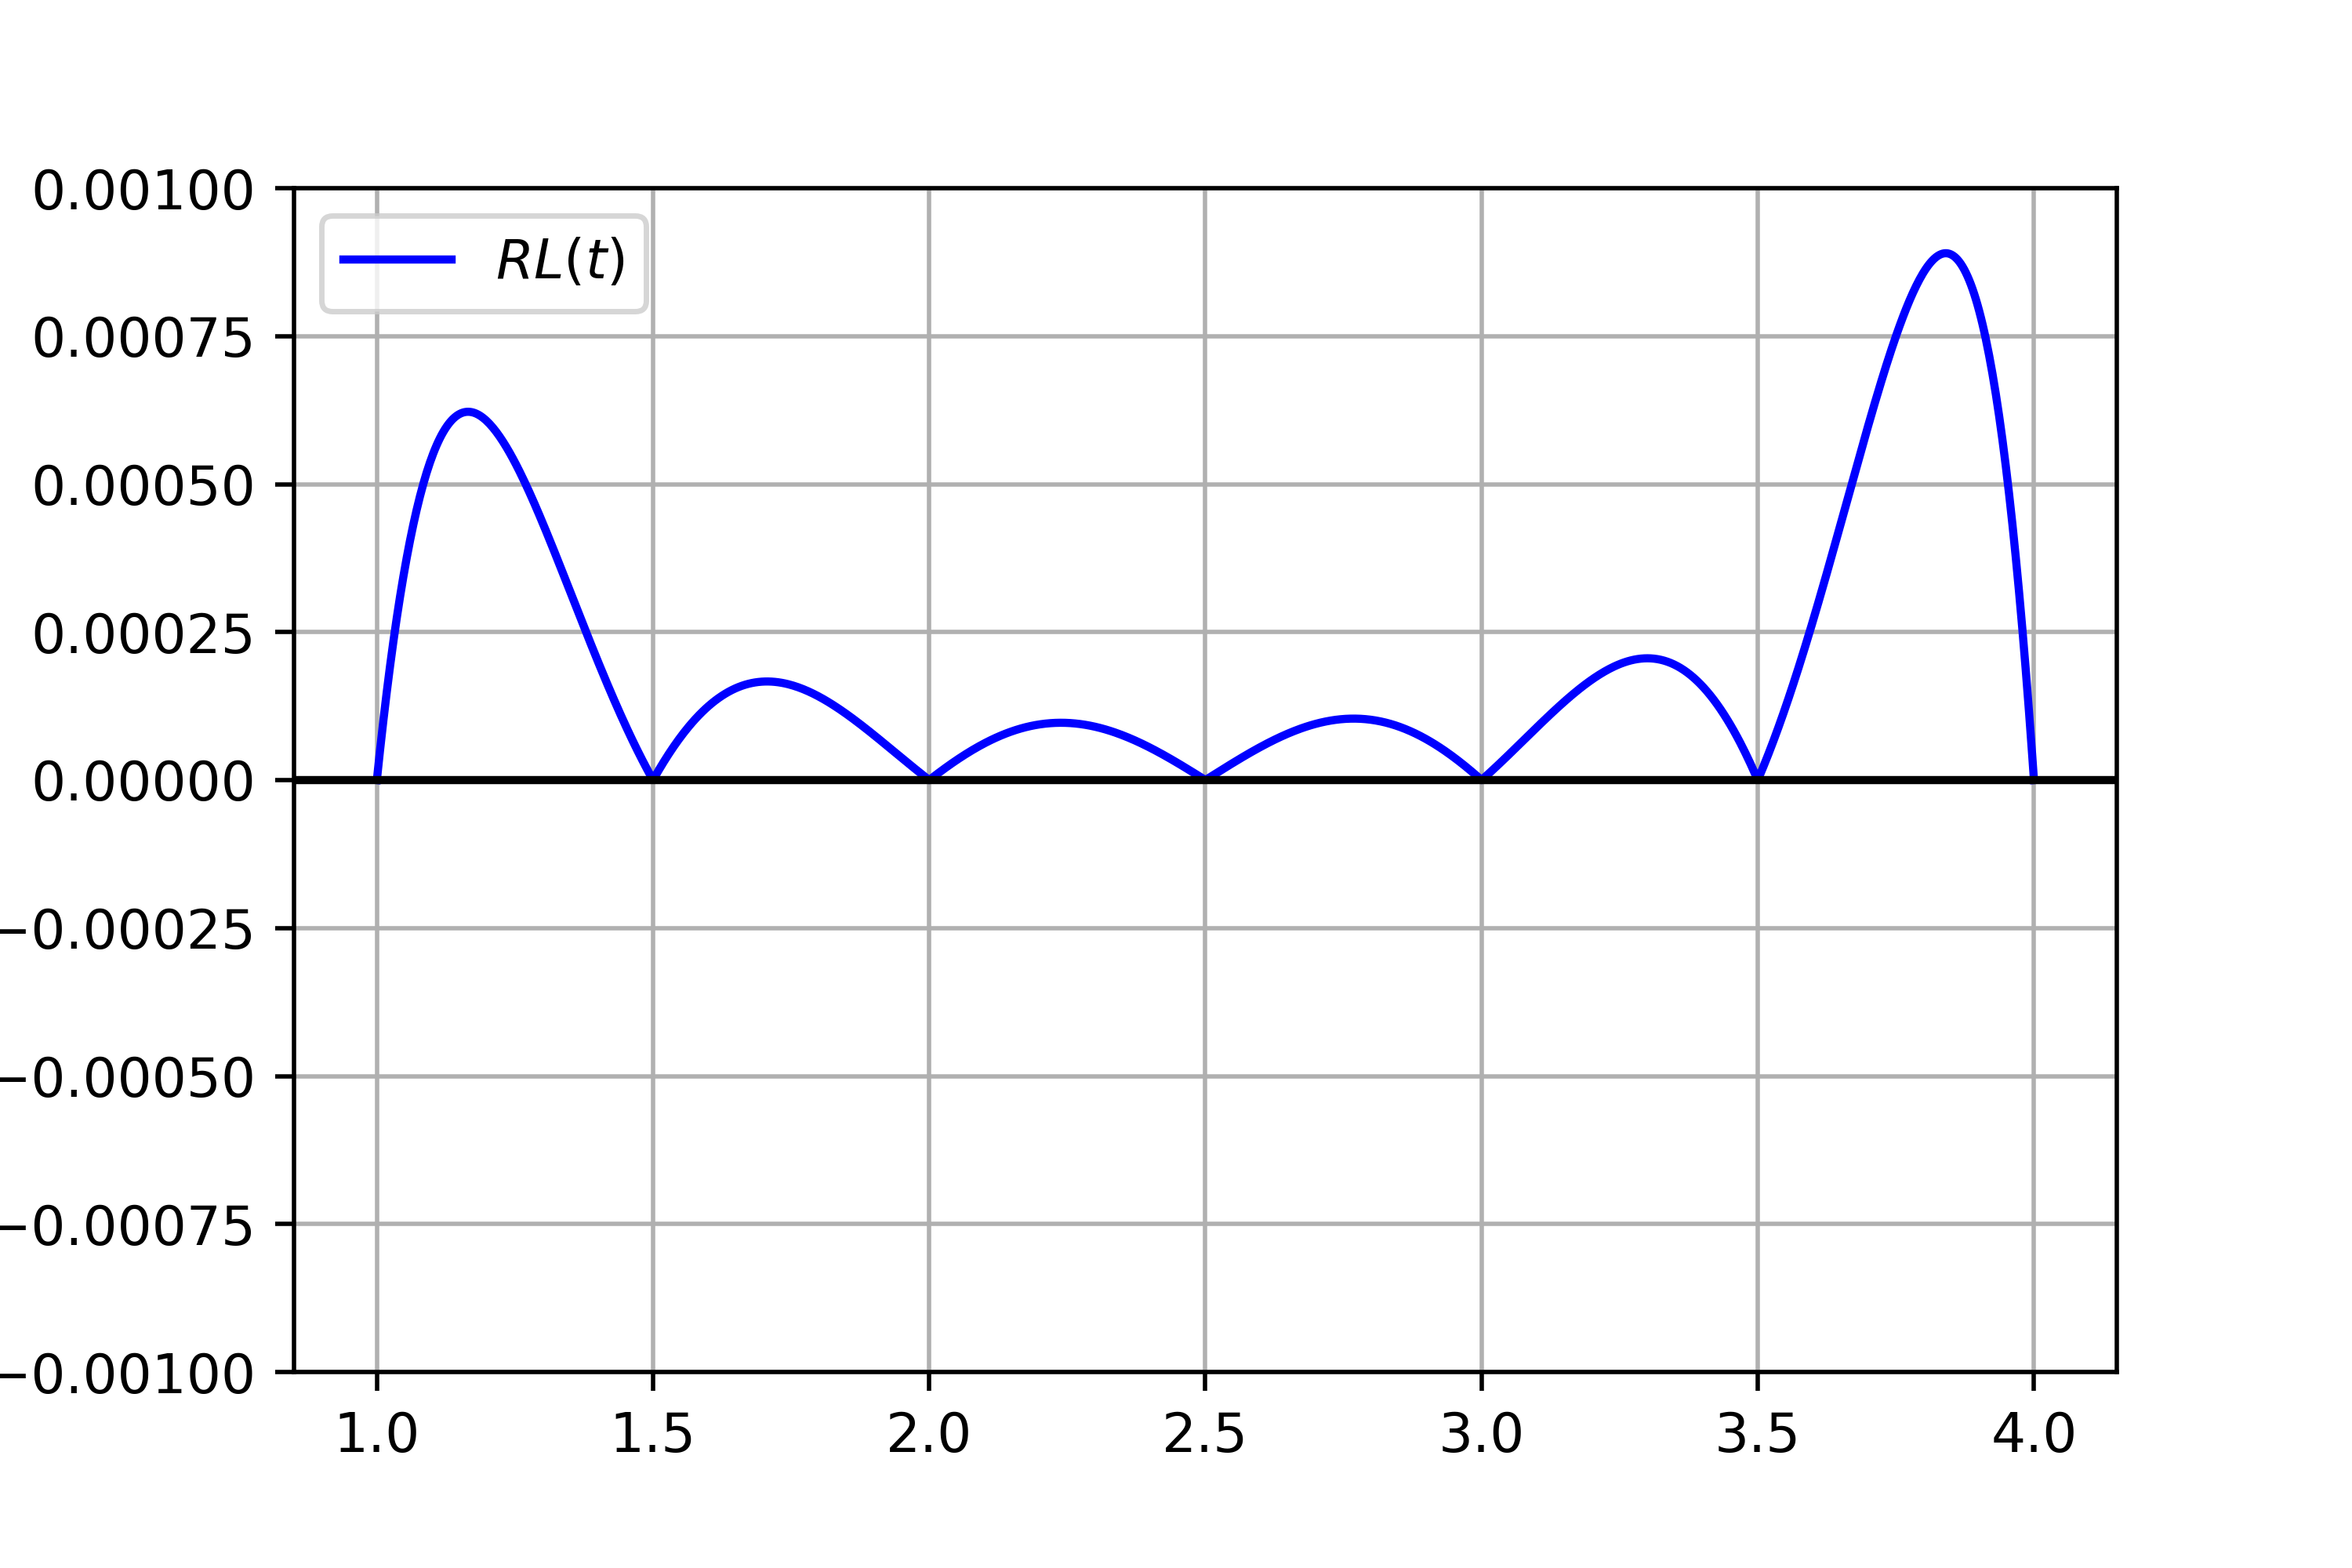
\includegraphics[width=8cm]{plot_4.2_err_Lagrange_equal.png}
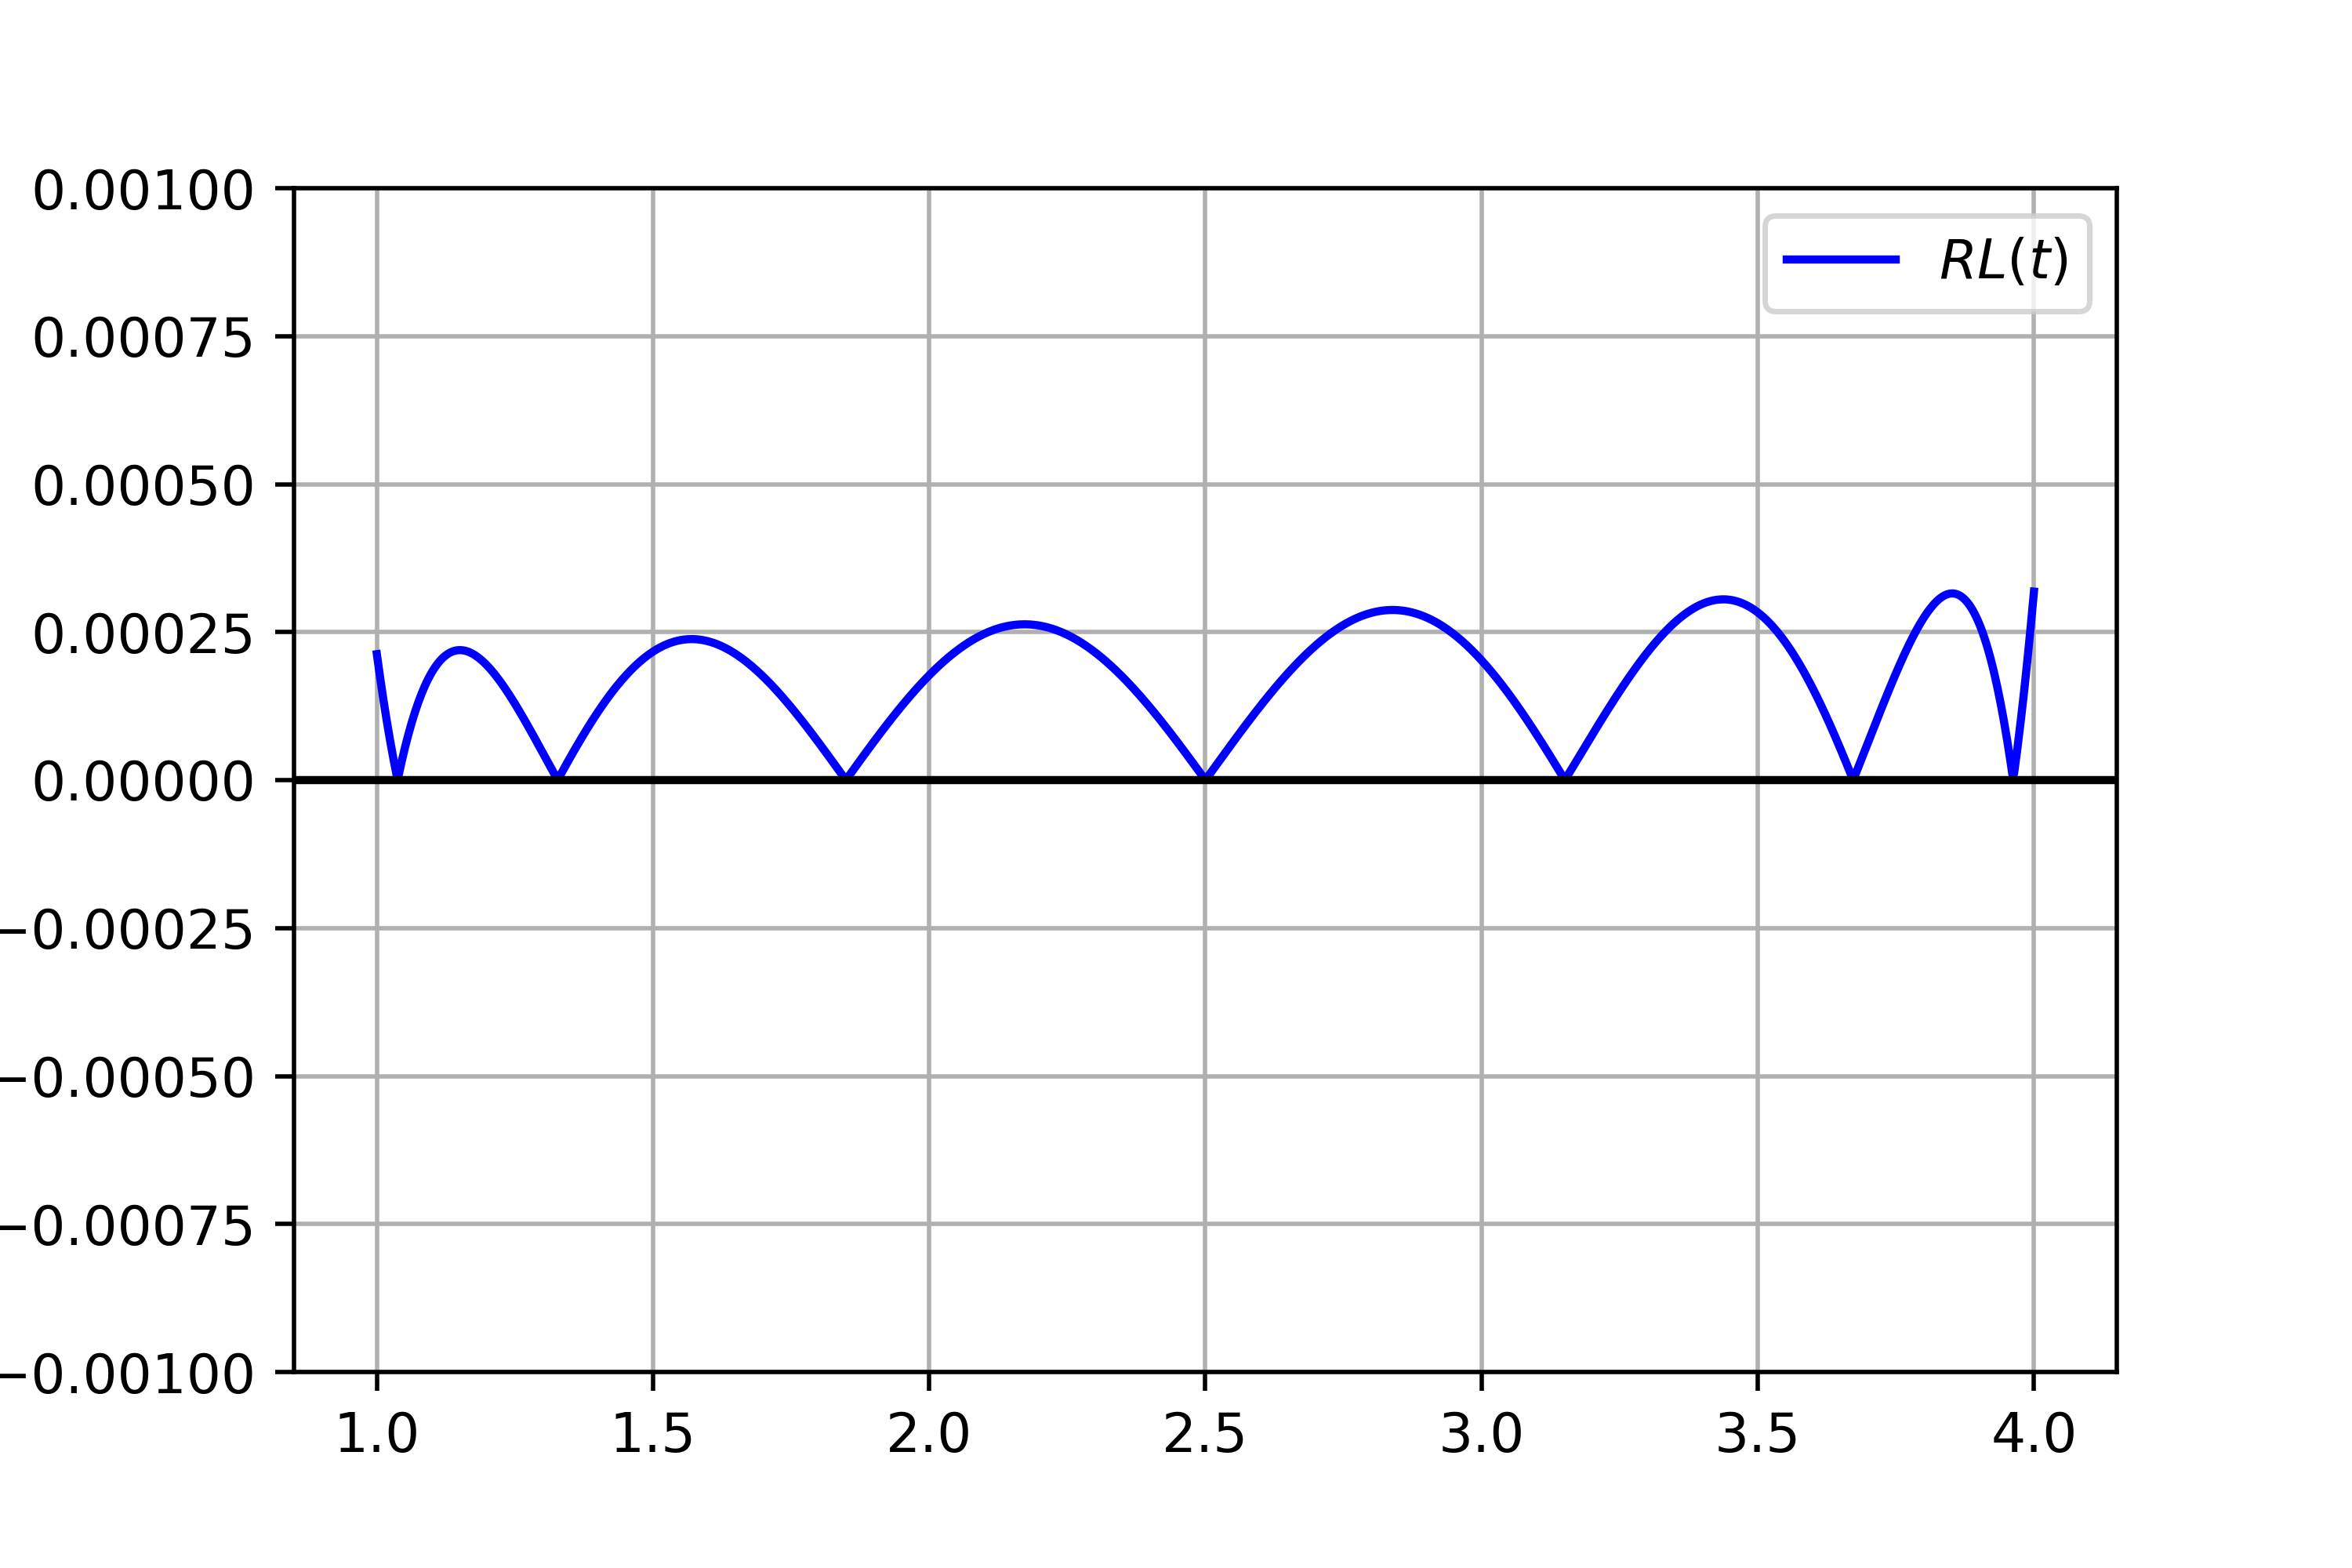
\includegraphics[width=8cm]{plot_4.2_err_Lagrange_Chebyschev.png}

Однако при приближении функции с помощью квадратичного сплайна наблюдается обратная ситуация - погрешность больше, если выбирать узлы соответственно нулям Чебышева (в обоих случаях $n = 69$):

\noindent
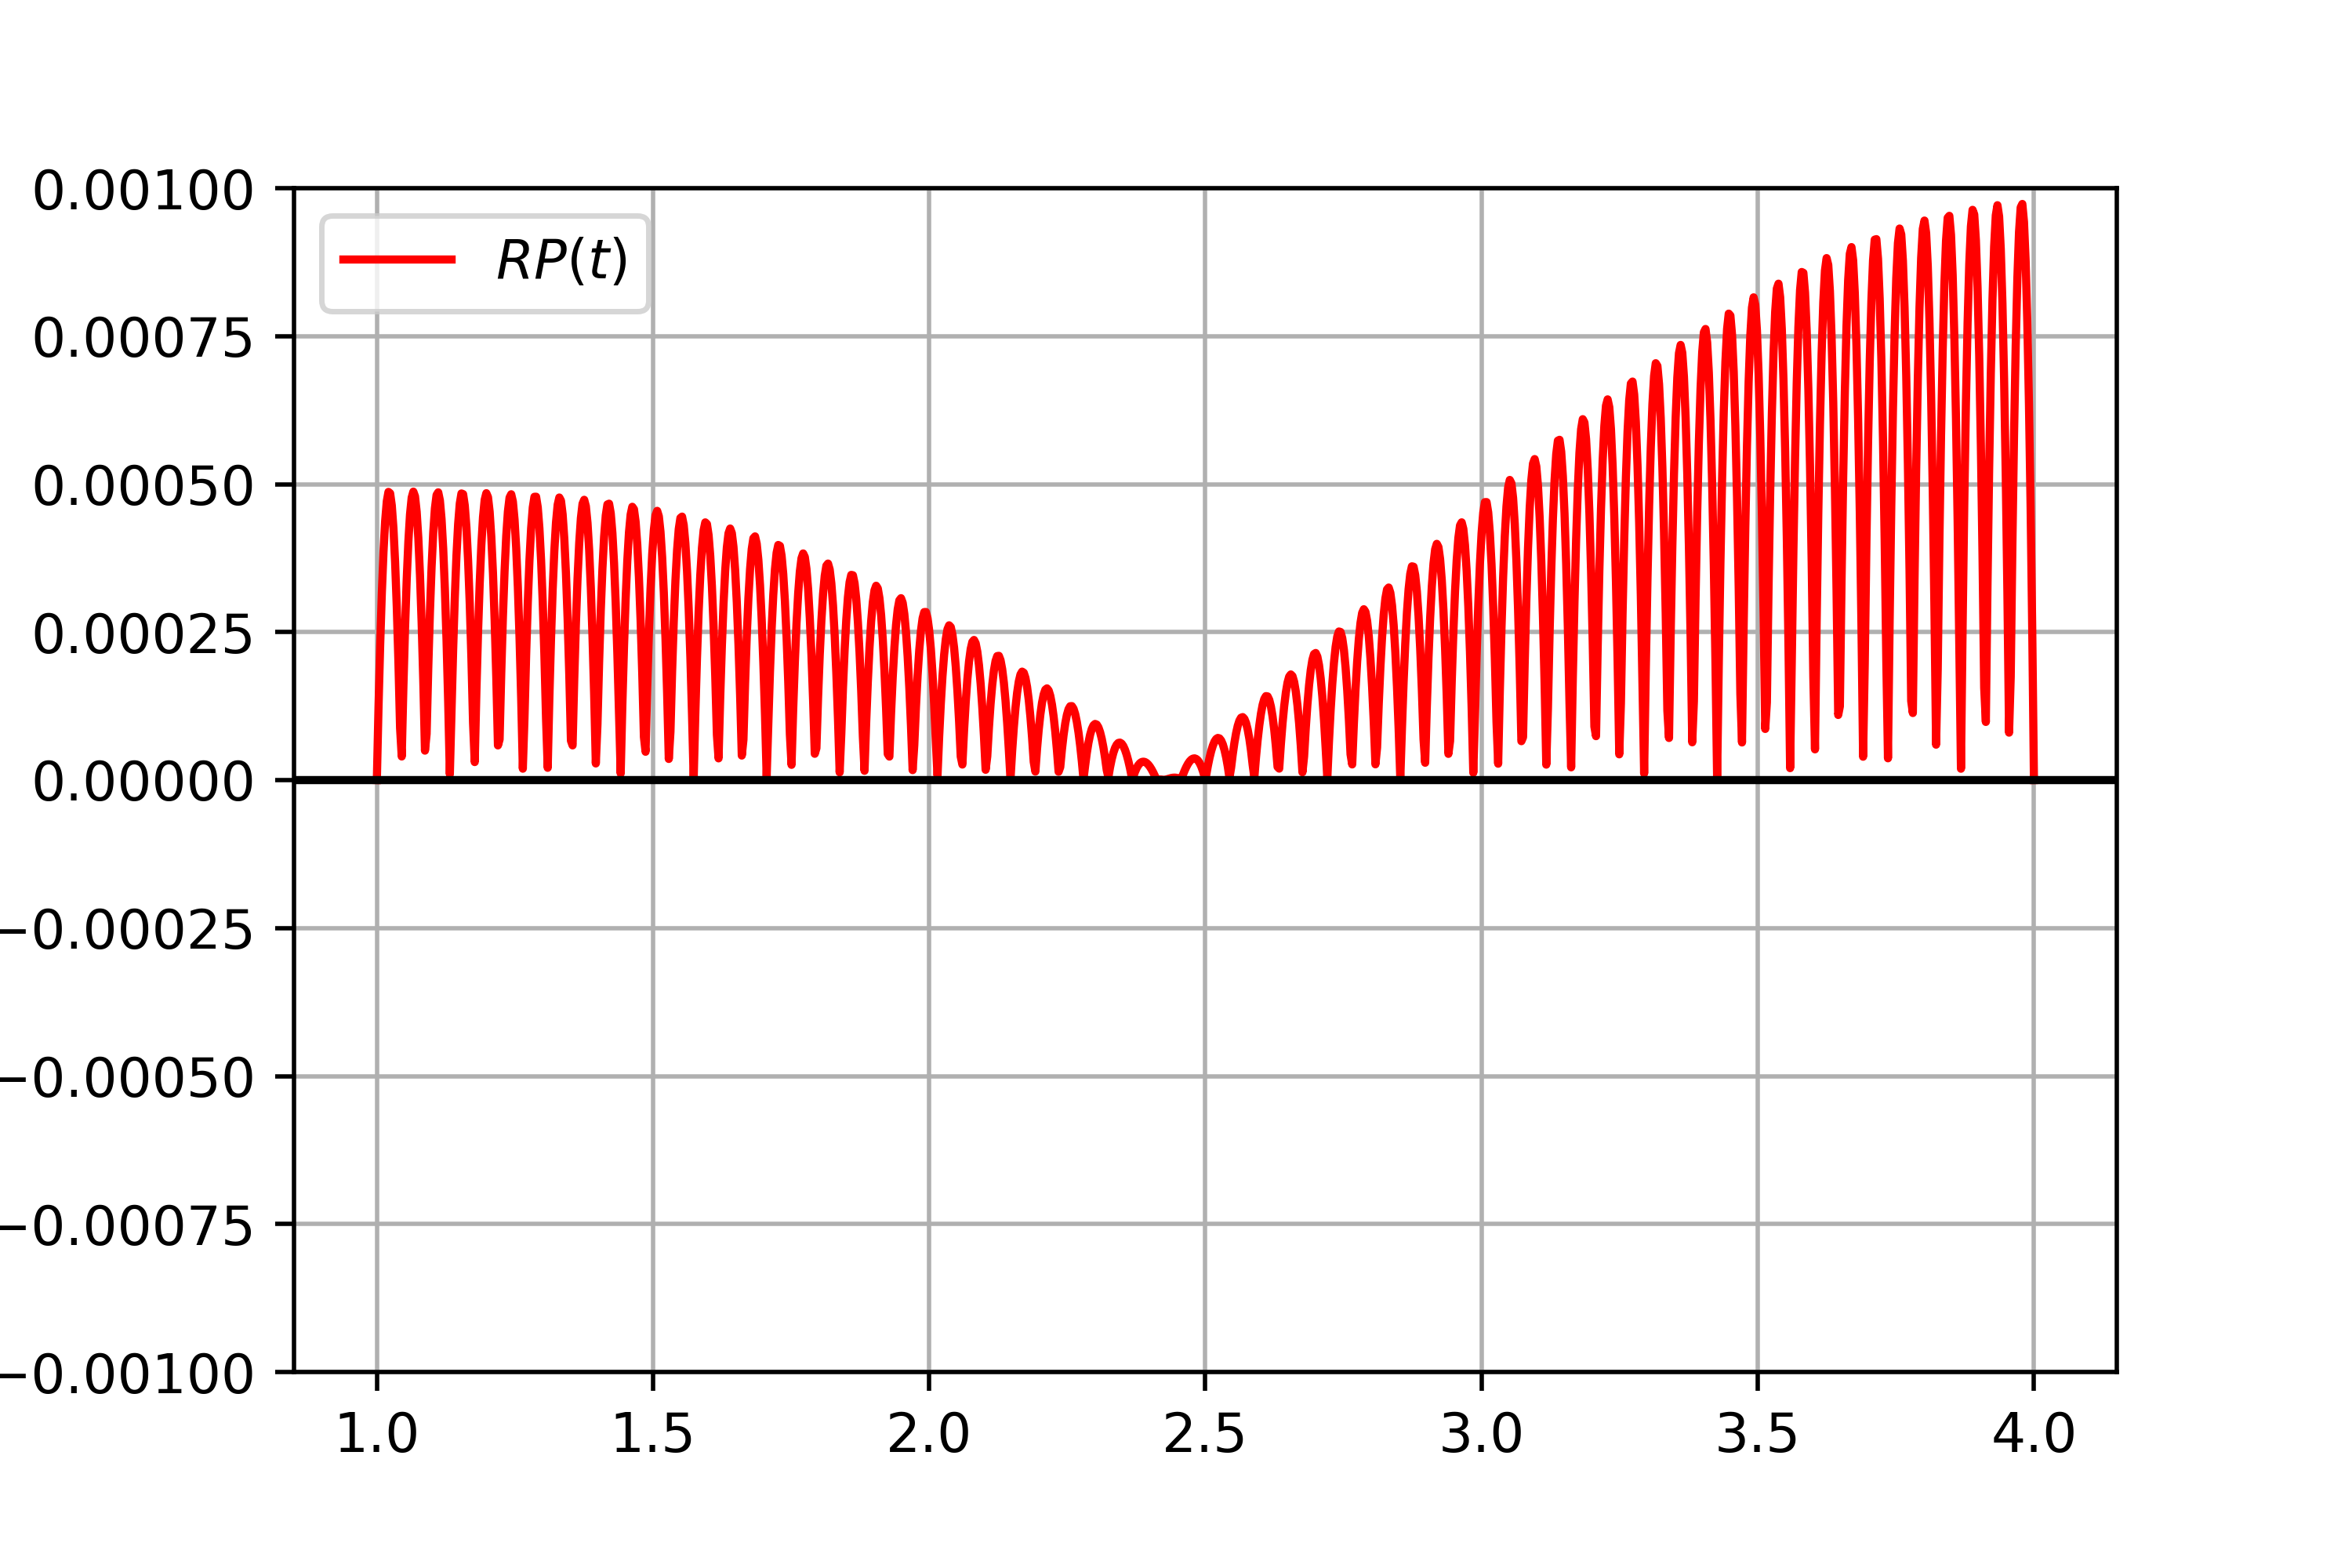
\includegraphics[width=8cm]{plot_4.2_err_Spline_equal.png}
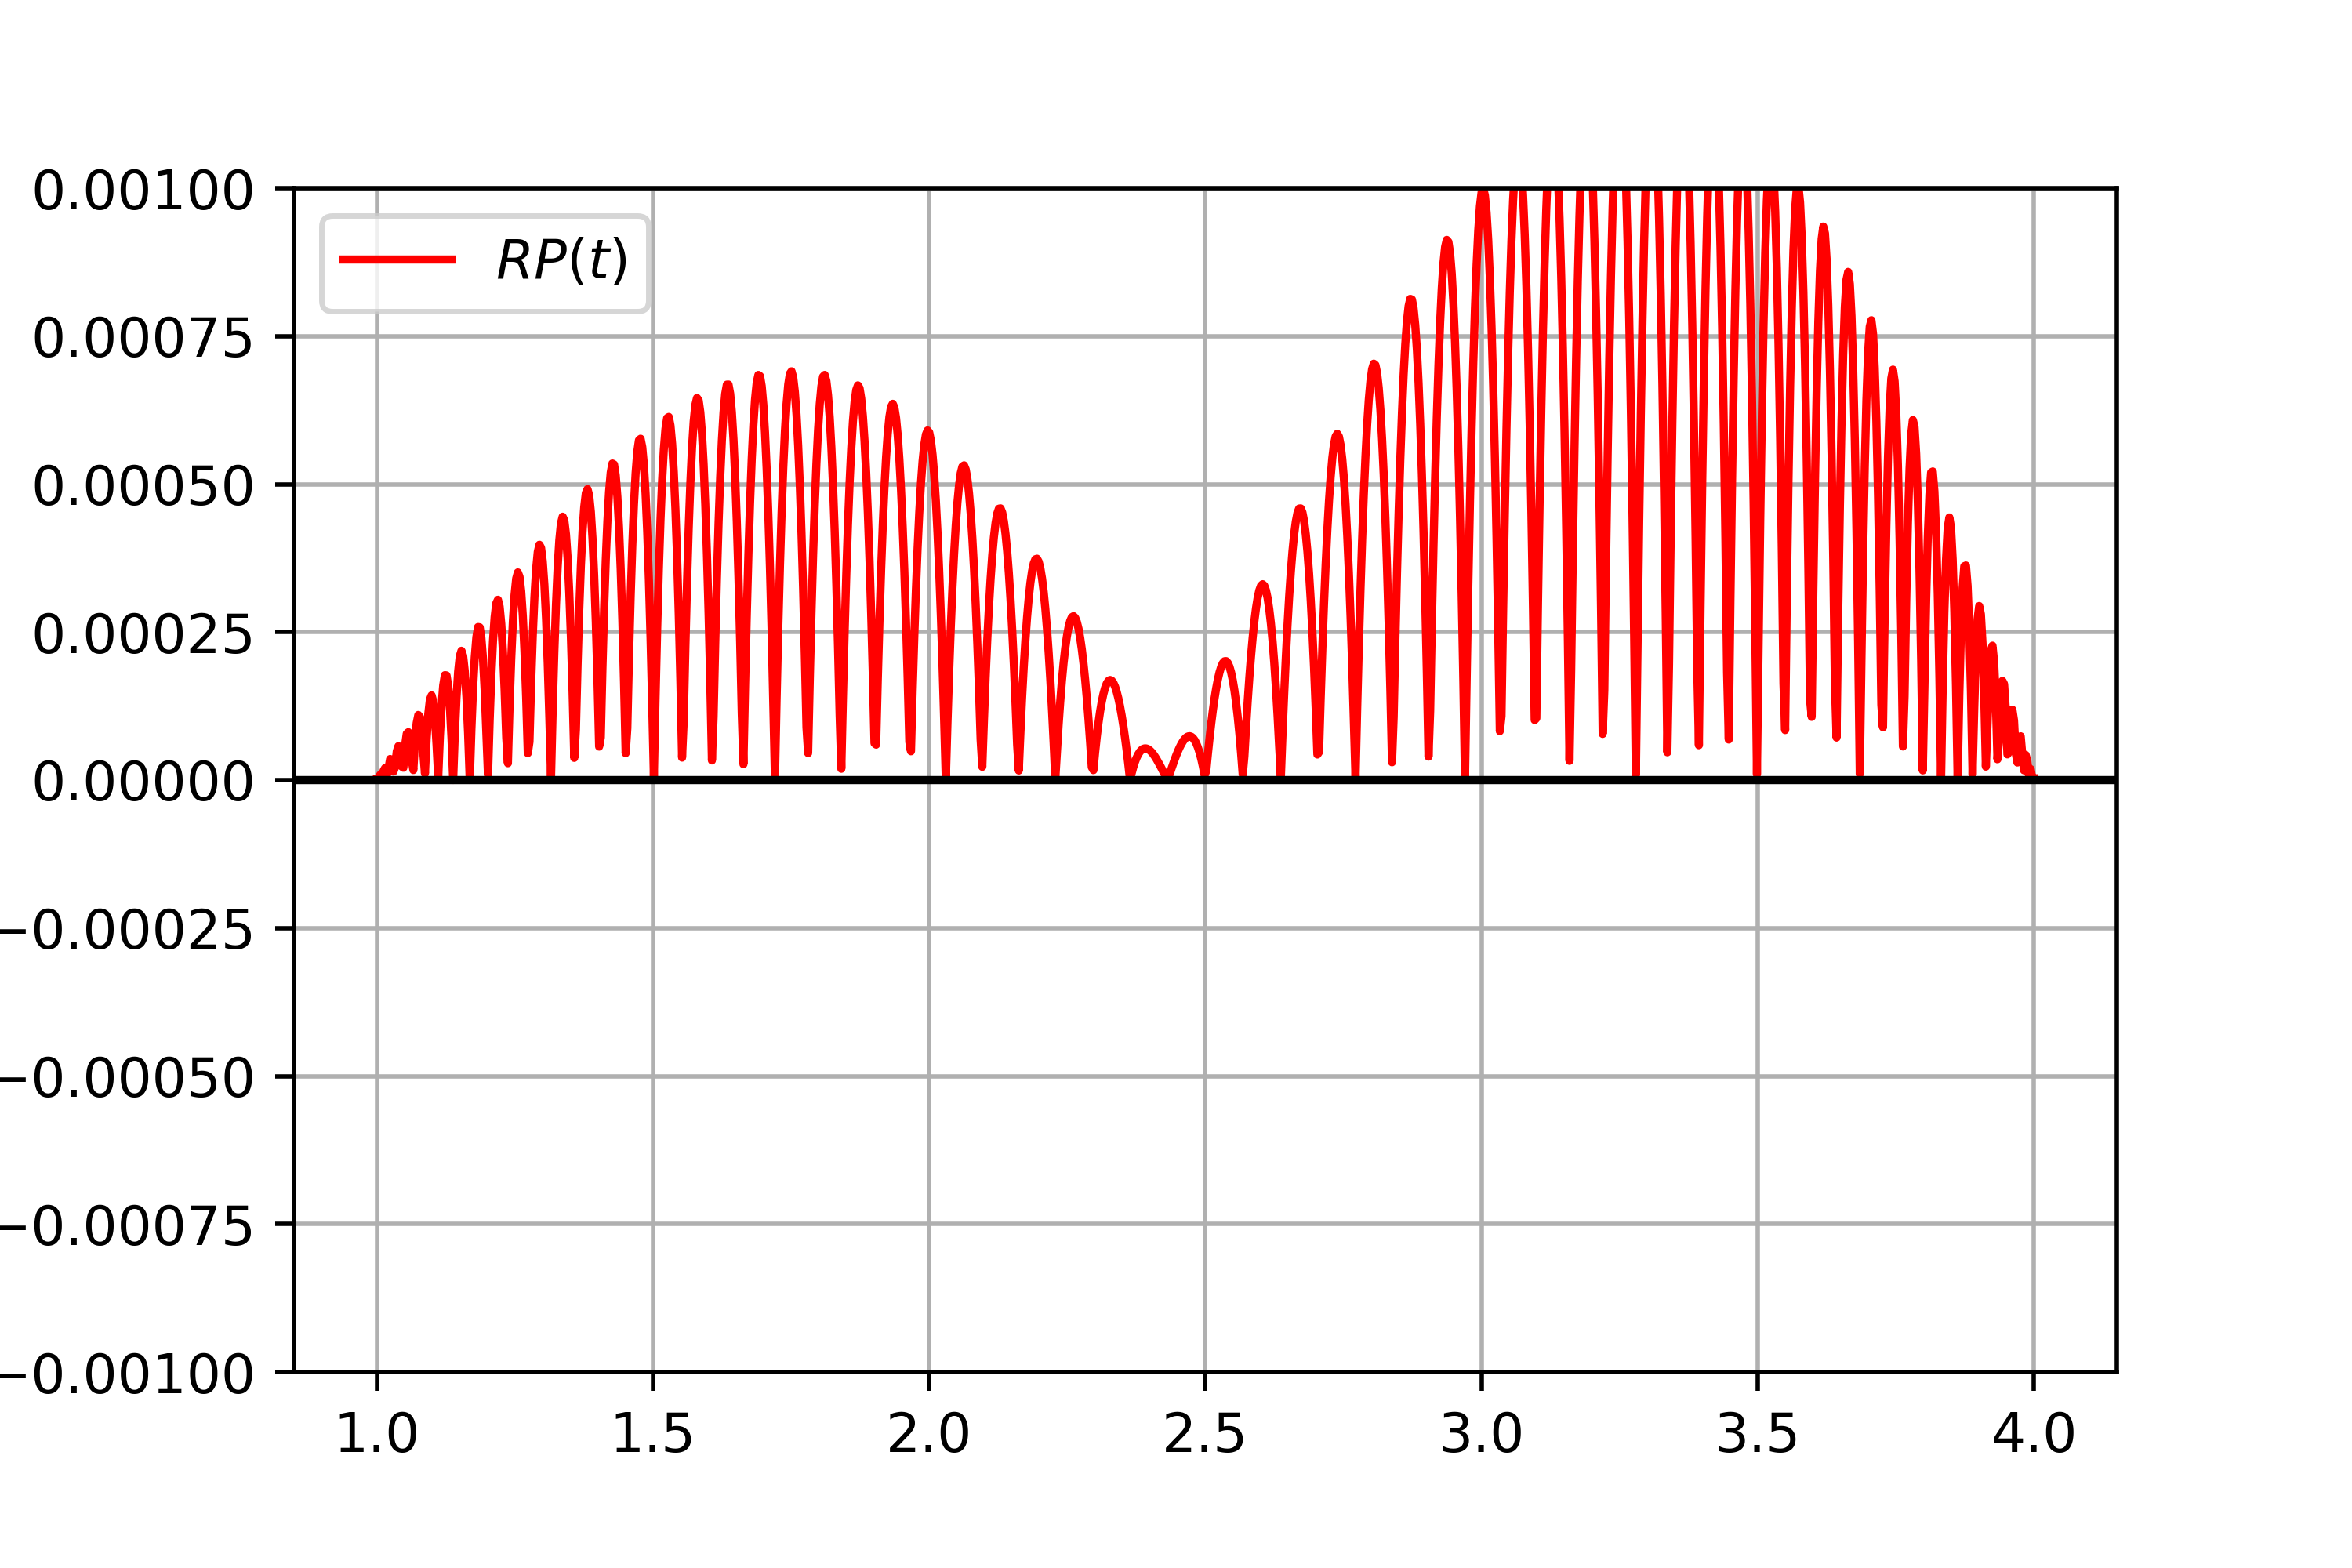
\includegraphics[width=8cm]{plot_4.2_err_Spline_Chebyschev.png}
\newline
Равномерный выбор узлов интерполяции
\hspace{1cm}По нулям Чебышева

Стоит отметить, что на обоих графиках явно выделяется точка, где обе погрешности минимальные - это точка перегиба, то есть где вторая производная равна нулю.

Ниже приведены графики многочлена Лагранжа($L(x)$), квадратичный сплайн ($P(x)$) и сама функция $f(x)$:

\noindent
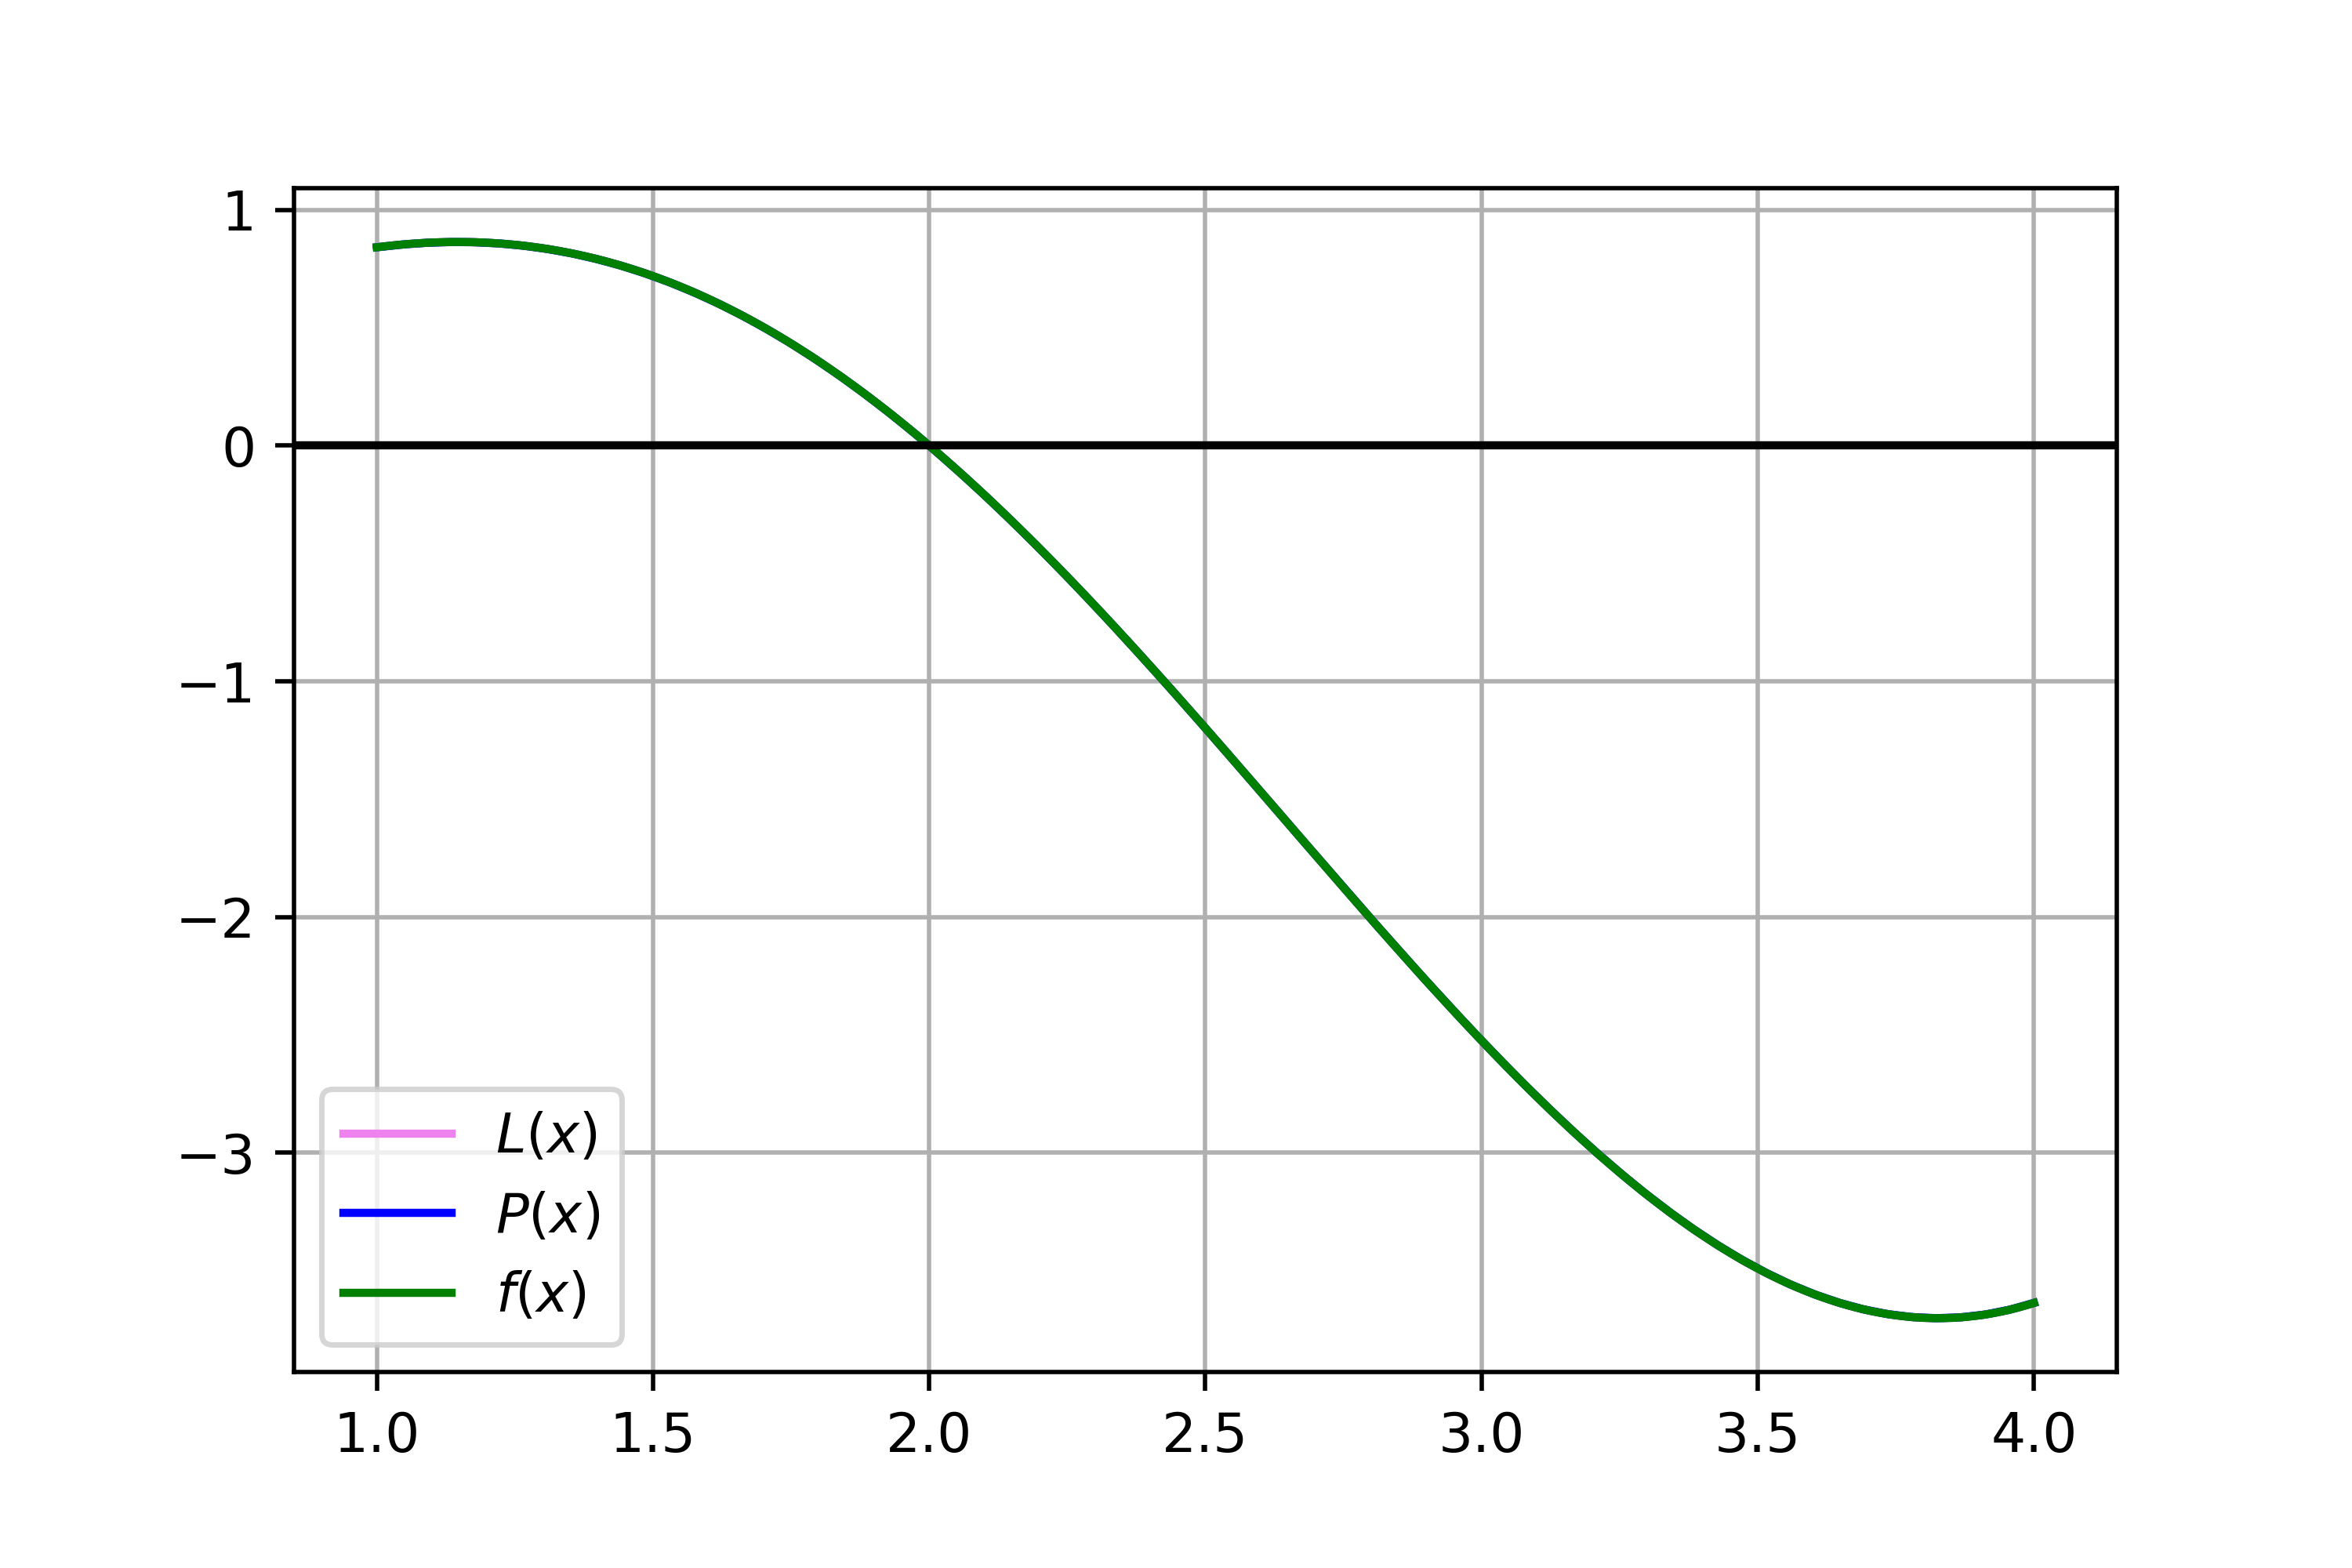
\includegraphics{plot_4.2_all_inter.png}

\subsection*{Код программы}
\begin{lstlisting}
import numpy as np
import matplotlib.pyplot as plt
from collections import namedtuple

def f(x: np.float64) -> np.float64:
    #return 1.0 / (1 + 25*x**2)
    return x*np.sin(2 - x)

def equal_partition(a: np.float64, b: np.float64, n: int) -> np.ndarray:
    return np.linspace(a, b, n)

def Chebyschev_partition(a: np.float64, b: np.float64, n: int) -> np.ndarray:
    n -= 1
    get_x = lambda k: 0.5*(a + b) + 0.5*(b - a) * np.cos(np.pi * (2*k + 1)/(2*n + 2))
    x = [get_x(k) for k in range(n, -1, -1)]
    partition = np.array(x)
    return partition

Polynom = namedtuple("Polynom", ["a", "b", "c", "x0", "x1"])
def make_spline(x: np.ndarray, y: np.ndarray, dfa: np.float64):
    spline = []
    n = len(x) - 1
    a, b, c = [0]*n, [0]*n, [0]*n
    for i in range(n):
        a[i] = y[i]
        b[i] = (y[i+1] - y[i]) / (x[i+1] - x[i])
    c[0] = (dfa - b[0])/(2*x[1])
    spline.append(Polynom(a[0], b[0], c[0], x[0], x[1]))
    for i in range(1, n):
        c[i] = (b[i] - b[i-1])/(2 * x[i+1]) + x[i-1]/x[i+1] * c[i-1]
        spline.append(Polynom(a[i], b[i], c[i], x[i], x[i+1]))
    return spline

a, b = 1, 4
n_dots = 69
x = equal_partition(a, b, n_dots) #100 0.005909864879679992
#x = Chebyschev_partition(a, b, n_dots) #100 0.007819083547945267
y = np.array([f(i) for i in x])
df1 = np.sin(1) - np.cos(1)
spline = make_spline(x, y, df1)

def Spline(arg: np.float64):
    n = len(spline)    
    if arg <= spline[0].x1:
        s = spline[0]
    elif arg >= spline[n - 1].x0:
        s = spline[n - 1]
    else:
        i, j = 0, n - 1
        while i + 1 < j:
            k = i + (j - i) // 2
            if arg <= spline[k].x0: j = k
            else: i = k
        s = spline[i]
    return s.a + s.b*(arg - s.x0) + s.c*(arg - s.x0)*(arg - s.x1)

x = Chebyschev_partition(a, b, 7)
y = np.array([f(i) for i in x])
def Lagrange_Polynom(arg):
    res = 0
    for i in range(len(x)):
        tmp = 1
        for k in range(len(x)):
            if i != k:
                tmp *= (arg - x[k])* 1.0/(x[i] - x[k])
        res += y[i]*tmp
    return res
\end{lstlisting}
